% chapters/04_ergebnisse.tex

\chapter{Ergebnisse}
\label{chap:ergebnisse}

\section{Trainingsverlauf}
\label{sec:trainingsverlauf}

\Cref{fig:loss-curve} zeigt den Verlauf der Verlustfunktion über
\num{[TODO]}~Trainingsschritte, aufgezeichnet mit \ac{wandb}.

\begin{figure}[htb]
  \centering
  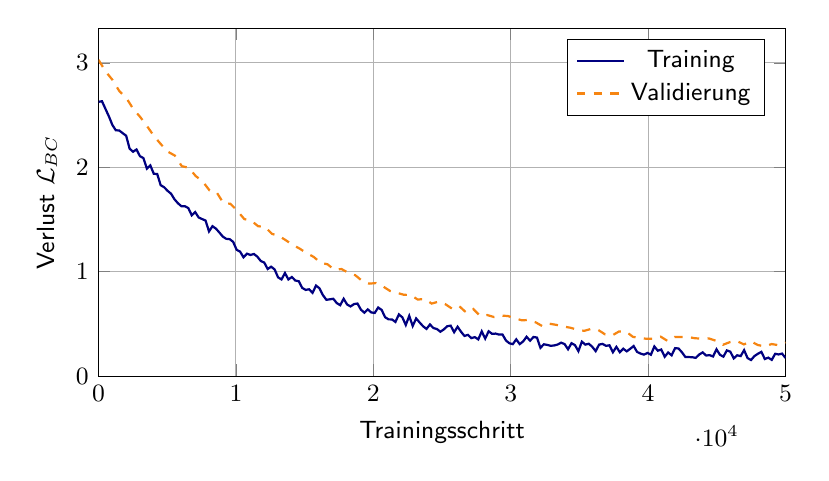
\begin{tikzpicture}
    \begin{axis}[
      width  = 0.85\textwidth,
      height = 6cm,
      xlabel = {Trainingsschritt},
      ylabel = {Verlust $\mathcal{L}_{\text{BC}}$},
      grid   = both,
      grid style = {line width=0.2pt, draw=gray!30},
      major grid style = {line width=0.4pt, draw=gray!60},
      xmin = 0, xmax = 50000,
      ymin = 0,
      xtick distance = 10000,
      legend pos = north east,
      legend style = {font=\small\sffamily},
      tick label style = {font=\small\sffamily},
      label style = {font=\small\sffamily},
    ]
      % Platzhalter-Kurve — durch echte Daten ersetzen:
      % \addplot[NavyBlue, thick] table[x=step, y=loss, col sep=comma]
      %   {data/training_log.csv};
      \addplot[NavyBlue, thick, domain=0:50000, samples=200]
        {2.5 * exp(-x/12000) + 0.15 + 0.05*rand};
      \addlegendentry{Training}

      \addplot[BurntOrange, thick, dashed, domain=0:50000, samples=100]
        {2.8 * exp(-x/14000) + 0.22 + 0.03*rand};
      \addlegendentry{Validierung}
    \end{axis}
  \end{tikzpicture}
  \caption{Trainingsverlust (Behavior Cloning) und Validierungsverlust über die
    Trainingsschritte. Platzhalter-Kurven — durch echte W\&B-Daten ersetzen.}
  \label{fig:loss-curve}
\end{figure}

\section{Evaluationsergebnisse}
\label{sec:evaluation}

Die Evaluation erfolgt anhand der Erfolgsrate beim Block-Stacking in der
Simulation (\emph{NVIDIA Isaac Lab}).
Insgesamt wurden $n = \num{[TODO]}$~Episoden pro Checkpoint ausgewertet
(\cref{tab:eval-results}).

\begin{table}[htb]
  \centering
  \caption{Evaluationsergebnisse verschiedener Checkpoints}
  \label{tab:eval-results}
  \begin{tabular}{rrrr}
    \toprule
    \textbf{Schritt} & \textbf{Erfolgsrate [\%]} &
    \textbf{Ø Episodenlänge [s]} & \textbf{Ø Griff-Fehler [mm]} \\
    \midrule
    \num{10000} & [TODO] & [TODO] & [TODO] \\
    \num{25000} & [TODO] & [TODO] & [TODO] \\
    \num{50000} & [TODO] & [TODO] & [TODO] \\
    \bottomrule
  \end{tabular}
\end{table}

\begin{infobox}[Erfolgsdefinition]
  Eine Episode gilt als erfolgreich, wenn alle Blöcke innerhalb von
  \qty{60}{\second} vollständig gestapelt sind und der Turm mindestens
  \qty{2}{\second} stabil bleibt.
\end{infobox}

\section{Ablation: Batch-Größe und Schritte}
\label{sec:ablation}

Um den Einfluss der Batch-Größe auf die Trainingseffizienz zu untersuchen,
wurden drei Konfigurationen verglichen (je~\num{25000}~Schritte):

\begin{figure}[htb]
  \centering
  \begin{tikzpicture}
    \begin{axis}[
      ybar,
      bar width    = 1.5cm,
      width        = 0.7\textwidth,
      height       = 5.5cm,
      ylabel       = {Erfolgsrate [\%]},
      symbolic x coords = {BS=8, BS=32, BS=64},
      xtick        = data,
      ymin         = 0, ymax = 100,
      ytick distance = 20,
      nodes near coords,
      nodes near coords align = {vertical},
      grid         = y,
      grid style   = {line width=0.3pt, draw=gray!40},
      tick label style = {font=\small\sffamily},
      label style  = {font=\small\sffamily},
      bar shift    = 0pt,
      fill         = NavyBlue!60,
      draw         = NavyBlue,
    ]
      % Platzhalter-Daten:
      \addplot coordinates {(BS=8,[TODO]) (BS=32,[TODO]) (BS=64,[TODO])};
    \end{axis}
  \end{tikzpicture}
  \caption{Einfluss der globalen Batch-Größe auf die Erfolgsrate nach
    \num{25000}~Schritten (Platzhalter-Werte).}
  \label{fig:ablation-batchsize}
\end{figure}
